\chapter{Extended Petri nets}\label{chapter:c3}
After introducing web services (and their composition) and the basic formalisms
that can be used to model and analyse them, we will focus on this chapter in defining the specific models used in this Thesis. Thus, we
will present some extensions of the basic model of Petri nets and some properties
that can be analysed. We will recall some notions (marking, firing, enabledness and so on) defined in the preceding chapter
and we will adapt them to a particular case. This chapter is mainly divided in two parts. On the one hand,
we will focus first on the definition of Coloured Petri nets since they are used in the definition of the language BPELRF, and, then,
we will present timed-arc Petri nets, in its two variants (discrete and continuous), as they are the basis of the workflow model presented in the
second part of the present Thesis.

\begin{definition} [(General Petri nets)]
A general Petri net is a 5-tuple $N=(P,T,F,K,W)$, where:
\begin{enumerate}
\item $(P,T,F)$ is a basic Petri net.
\item $K\,:\,P \longrightarrow \nnul \,\cup\, \{\infty\}$ is a function that
indicates the maximum number of tokens in each place (capacity function).
\item $W\,:\,F \longrightarrow \nnul$ is a function that indicates
the multiplicity of the arcs ({\it weight of the arcs}).
\end{enumerate}
When the context is clear, we will call them Petri nets. The function $K$
can be omitted if it is infinite for all the places in the net.
%Adem\'{a}s, es
%usual extender la definici\'{o}n de $W$ a todo el universo de
%posibles arcos, haci\'{e}ndola nula para pares
%$(p,t)$ o $(t,p)$ que no est\'{e}n en $F$.
\end{definition}

\begin{definition} [(Firing rule for general Petri nets)]
Let $N=(P,T,F,K,W)$ be a general Petri net.
\begin{enumerate}
\item A function $M\,:\, P \longrightarrow \nnul$ is a marking
$N$ iff $M(p) \leq K(p)$, for all
$p \in P$.
\item A transition $t \in T$ is enabled in $M$, denoted by $M[ t \rangle$,
iff $W(p,t) \leq M(p)$ and  $K(p) \leq M(p)-W(p,t)+W(t,p)$, for all $p \in P$.
The firing of $t$ produces the marking $M'$:
$M'(p) = M(p) - W(p,t) + W(t,p)$, for all $p \in P$.
Again, this evolution is denoted by $M[ t \rangle M'$.
\item A multiset of transitions $R$ is enabled in $M$, written $M [ R \rangle$, if and only if
$M(p) \geq \sum_{t \in T} W(p,t) \cdot R(t)$. The firing of $R$,  denoted by $M [ R \rangle M'$,
produces $M'$:
\[ M'(p) = M(p) - \sum_{t \in T} (W(p,t) - W(t,p)) \cdot R(t), \,\,
\forall p \in P\]
\end{enumerate}
\end{definition}

\begin{definition} [(Occurrence Sequence)]
Let $N=(P,T,F,K,W,M_0)$ be a marked Petri net.
\begin{enumerate}
\item $\sigma = M_0 t_1 M_1 \ldots t_n M_n$ is a finite occurrence sequence of $N$
if and only if $\forall i \in \{1,\ldots,n\},\,M_{i-1} [ t_i \rangle M_i$.
Occasionally, we will write $t_1 \ldots t_n$, omitting the corresponding markings, since starting from
$M_0$ it is easy to obtain the rest of the markings knowing the transitions fired.
We extend the conventional notation to occurrence sequences, 
obtaining $M_0 [ \sigma \rangle M_n$.
The set of occurrence sequences starting from $M_0$ are denoted by $L(N,M_0)$.

\item For multiple transitions, $\sigma = M_0 R_1 M_1 \ldots R_n M_n$ is a finite step sequence
iff $\forall i \in \{1,\ldots,n\}$, $\,M_{i-1} [ R_i \rangle M_i$.
%Again, we extend the notation to occurrence sequence, $M_0 [ \sigma \rangle M_n$.
The set of finite step sequences of $N$ starting from $M_0$ is denoted by $P(N,M_0)$.
\end{enumerate}
\end{definition}

%En lo sucesivo trabajaremos usualmente sobre la sem\'{a}ntica de
%secuencias de ocurrencia, salvo que expl\'{\i}citamente se
%indique lo contrario.

%\bdfn (Matrices de Incidencia)\\
%Sea $N=(P,T,F,W,M_0)$ una Red de Petri Marcada.
%\begin{enumerate}
%\item Se dice que $N$ es {\it pura} sii $\forall t \in T$,
%$\forall p \in P$, $W(t,p) \cdot W(p,t) = 0$.
%\item Si $N$ es una red pura, podemos definir su
%{\it matriz de incidencia previa}, $C^{-} = (c_{i,j}^{-})$,
%$i=1,\ldots,|P|\,;\,j=1,\ldots,|T|$, siendo
%$c_{i,j}^{-} = W(p_i,t_j)$, y su
%{\it matriz de incidencia posterior}
%$C^{+} = (c_{i,j}^{+})$,
%$i=1,\ldots,|P|\,;\,j=1,\ldots,|T|$, siendo
%$c_{i,j}^{+} = W(t_i,p_j)$.
%\item Si $N$ es una red pura se define su {\it matriz de
%incidencia} $C$ por medio de $C = C^+ - C^-$.
%\end{enumerate}
%\edfn

%La matriz de incidencia puede ser definida tambi\'{e}n sobre redes
%que no sean puras, pero en tal caso no caracteriza a las mismas, pues
%una misma matriz de incidencia corresponde a varias redes diferentes.
%
%\bex Es sencillo obtener dos Redes de Petri diferentes con la misma
%matriz de incidencia. Para ello basta tomar
%una Red de Petri Ordinaria y elegir un lugar y una transici\'{o}n
%no conectados inicialmente, y conectarlos formando un loop. Por
%ejemplo, las dos redes de la figura \ref{fig203} tienen la misma
%matriz de incidencia. De hecho, si se trabaja con Redes Generalizadas
%el a\~{n}adido se puede hacer sobre cualquier par.
%\eex
%
%\begin{figure}
%\input{fig28}
%\caption{\label{fig203} Dos Redes de Petri con la misma Matriz de Incidencia}
%\end{figure}

%\bprop (Ecuaci\'{o}n de Estado)\\
%Sea $N=(P,T,F,W,M_0)$ una Red de Petri Marcada Pura,
%$\sigma \in L(N,M_0)$, y $M_0 [ \sigma \rangle M$.
%Entonces se tiene: $M = M_0 + C \cdot \bar{\sigma}$, siendo
%$\bar{\sigma}$ el vector de Parikh asociado a la
%secuencia $\sigma$, que est\'{a} definido como
%$\bar{\sigma}(i) = $n\'{u}mero de ocurrencias de
%la transici\'{o}n $t_i$ en la secuencia $\sigma$.
%
%\proof Sea la secuencia de marcajes producida a lo
%largo de la ejecuci\'{o}n de $\sigma$: $M_0 t_{i_{1}} M_1 \ldots t_{i_{n}} M_n$.
%Entonces, de la regla de disparo se concluye que $M_1 = M_0 +
%C \cdot U_{i_{1}}$, siendo $U_{i_{1}}$ el vector cuyas componentes son todas
%nulas, salvo la $i_{1}$-\'{e}sima, que vale 1. En general, se obtiene
%que $M_k = M_{k-1} + C \cdot U_{i_{k}}$.
%
%Por tanto:
%\[ M_k = M_{k-2} + C \cdot (U_{i_{k-1}} + U_{i_{k}}) = \ldots =
%M_0 + C \cdot \sum_{j=1}^{k} U_{i_{j}}\]
%Ahora bien, $\suma{j=1}{k} U_{i_{j}} = \bar{\sigma}$, lo que
%termina la demostraci\'{o}n.
%\eprop

\section{Petri nets analysis}
When designing a new system, the construction of a graphical model (e.g. a Petri net) of it is always
helpful since it is interesting to broadly understand how this system works before building it. This also helps designers to have a
deeper knowledge about how it evolves in its different steps. Nevertheless, the presence of a graphical model is not enough in many cases
as the designers want the system to meet some properties of interest. For instance, the system can be useless
if it can become deadlocked in some executions. To this end, it is valuable to have tools that allow to
evaluate properties in the model (and, in extension, in the real system). In finite sequential systems, 
it is not particularly challenging to check
the fulfilment of certain statement, whereas the presence of concurrency complicates this task.
Thus, the analysis of system behaviour is intended to determine the compliance of 
certain properties such as that the number of processes in a queue does not exceed
certain threshold or that the mutual exclusion is guaranteed when accessing to a shared resource.

In Petri nets, one can use a set of powerful tools to formally analyse
the compliance of such properties. With these tools, designers can check
the absence of deadlocks, the reachability of a certain
state, the possibility of reaching a concrete situation after performing some computations and so on.
Some examples of these tools are TINA \cite{TINA}, CPNTools, \cite{CPNTools}, Snoopy \cite{Snoopy} and GreatSPN \cite{GreatSPN}.

\medskip
Normally, these properties are divided in two categories: % Incluir cita si se encuentra

\subsection{Safety properties}
A safety property asserts that \emph{``nothing bad happens''}.
Thus, they guarantee that a set of undesirable states are not reached or that
the system does not execute an unwanted occurrence sequence.

The \emph{safety properties} are the following:

\begin{enumerate}
\item {\bf Reachability}. A marking $M$ of a marked Petri net
$N= (P,T,F,W,M_0)$ is {\it reachable} in $N$
iff there exists an occurrence sequence $\sigma \in L(N,M_0)$
such that $M_0 [ \sigma \rangle M$. We will denote by $[M_0\rangle$ the
set of reachable markings of $N$ starting from $M_0$, and
by $[ M \rangle$ the set of reachable markings starting from the marking $M$.

\item {\bf Boundedness}. A marked Petri net $N=(P,T,F,W,M_0)$ 
is {\it k-bounded}, for some $k \in \nnul$, if for all reachable marking
$M$ from $M_0$, it holds $M(p) \leq k$, for all $p \in P$. $N$ is said to be safe if
it is 1-bounded. A place $p \in P$ is
{\it n-safe} if $M(p) \leq n$, for all marking $M$ reachable from $M_0$.

%\item {\bf Boundedness}. Sea
%$N=(P,T,F,W,M_0)$ una Red de Petri Marcada.
%Se dice que un lugar $p \in P$ es limitado si
%existe un n\'{u}mero natural $n \in \nnul$ tal que dicho lugar es
%$n$-seguro; y se dice que $N$ es {\it limitada} si todos sus lugares
%son limitados.
\item {\bf Deadlock-free}. Let $N=(P,T,F,W,M_0)$ a marked Petri net and $M$ be a reachable marking.
$M$ is a {\it dead marking} if there is no $t \in T$ enabled at $M$. 
The net $N$ is deadlock-free iff there are no dead markings.

%\item {\bf Conservaci\'{o}n Respecto a un Vector de Pesos}.
%Sea una Red de Petri Marcada $N=(P,T,F,W,M_0)$, con
%$P = \{p_1,\ldots,p_n\}$. Se dice que $N$ es
%{\it conservativa respecto a un vector de pesos w}, con
%$w \in \nnul^n$, si para todo marcaje alcanzable $M$
%a partir de $M_0$ se cumple:
%\[ \suma{i=1}{n} w_i \cdot M(p_i) =
%\suma{i=1}{n} w_i \cdot M_0(p_i)\]
\item {\bf Coverability}.
Let $N=(P,T,F,W,M_0)$ be a marked Petri net and $M$ be a marking of $N$.
$M$ is said to be {\it coverable} if there exists $M' \in
[M_0 \rangle$ such that $M'(p) \geq M(p)$, for all $p \in P$.
\end{enumerate}

%\noindent {\sc NOTA:} Para ser m\'{a}s precisos, la alcanzabilidad no es
%exactamente una propiedad de seguridad, sino la negaci\'{o}n de la propiedad,
%la no alcanzabilidad. An\'{a}logamente ocurre con el cubrimiento de marcajes.

\subsection{Liveness properties}
A liveness property asserts that \emph{``something good eventually happens''}.
For instance, they guarantee that, independently of the current state of the system,
a specific state can eventually be reached or that a certain occurrence sequence can eventually
be executed in the system.

The \emph{liveness properties} are:
\begin{enumerate}
\item {\bf Liveness}.
Let $N=(P,T,F,W,M_0)$ be a marked Petri net. A transition $t \in T$
is said to be {\it live} if for all reachable marking $M \in
[ M_0 \rangle$ there is an occurrence sequence $\sigma$ starting from $M$ such that
$\sigma = t_1 \ldots t_m$, with $t_m = t$. The net $N$ is {\it live} iff all the transitions are live.
\item {\bf Home State}.
Let $N=(P,T,F,W,M_0)$ be a marked Petri net. A marking $M$ of $N$ is a {\it home state} if for all
$M' \in [ M_0 \rangle$, $M \in [ M' \rangle$.
\item {\bf Home Space}. Let $N=(P,T,F,W,M_0)$ be a marked Petri net.
The set of markings ${\cal M}$ is a {\it home-space}
of $N$ if for all marking $M' \in [ M_0 \rangle$ there is a marking
$M'' \in {\cal M}$ such that $M'' \in [ M' \rangle$.
\item {\bf Cyclic}.
Let $N=(P,T,F,W,M_0)$ be a marked Petri net. It is said that
$N$ is cyclic if for all marking $M \in [ M_0 \rangle$ there exists an occurrence sequence $\sigma$
starting at $M$ such that $M [ \sigma \rangle M_0$.
\end{enumerate}


% %JIRI % % % %



\section{Timed extensions of Petri nets}

In the
literature on timed extensions for Petri nets we can identify a
first group of models, which assign time delays to transitions,
by using either a fixed deterministic value
\cite{Ram74,Sif77,VFC93} or choosing it from a probability
distribution \cite{AjCh85}. Other models use time intervals to
establish the enabling times of transitions \cite{Mer74}. 
There are also models that include time on tokens
\cite{van93,van95,BLT90}. In \cite{Bow96,Wan98} 
a summary of time extensions for Petri nets is presented.

%Nota.- Extender un poco mas esto con información de cada paper

In PTCPNs, places have an associated colour set (data types). 
Each token has then an attached data value
({\em token colour}),
which belongs to the colour to which the token is
associated. We will use timed colours, for which the first component
will be a non-negative integer value, representing the data value,
and the second component will be the token timestamp,
a natural number representing the time at which the 
token will be available.

There is also a discrete global clock that represents
the total time elapsed in the system model. Moreover, arcs have also 
an associated inscription ({\em arc expressions}),
constructed using variables, constants, operators
and functions. 
To evaluate an arc expression we need to
bind the variables that are part of the expression with their current value, that is, this binding
consists of assigning a value to the variables that appear in the
arc inscription. These values are then used to
select the token colours that must be removed or added when
firing the corresponding transition.

Arc expressions can also have associated time information
both for place-transition and transition-place arcs.
However, only time inscriptions are needed
in output arcs, and even, when all the output arcs
of a transition have the same time inscription,
there is a shorthand notation in CPN Tools
by which this time information is associated with
the transition instead of the output arcs.

The time inscription associated with a transition 
is used to specify the delay that must be added to the
current value of the global clock for
every token generated by the firing of the transition.

Transitions can also have associated guards, which
are Boolean expressions that can prevent their firing.
Thus, when a transition has a guard, it must evaluate to
true for the binding to be enabled,
otherwise the binding is disabled and 
the transition cannot be fired. 

\begin{definition} [(Prioritised-Timed Coloured Petri Nets)]\label{ptcpndef}
A prioritised-timed coloured Petri net is a tuple \ptcpntuple, where: %\footnote{
%We use the classical notation on Petri nets to denote the
%precondition and postcondition of both places and transitions:
%%
%\[ \forall x \in P\,\cup\,T\,:\,
%\precond{x} = \{ y \,|\, (y,x) \in A\}~~~~~
%   x^{\bullet} = \{ y \,|\, (x,y) \in A\}
%\]
%}:
%%
\begin{itemize}
\item $P$ is a finite set of {\em places}, with colours
in the set $\Sigma$. Thus, in our case, colours 
will be pairs $(n,x)\in \nnul \times \nnul$, where $n$ is
the token value and $x$ its timestamp.
%
\item $T$ is a finite set of {\em transitions} ($P\cap T = \emptyset$).
%
\item $A \subseteq (P\times T)\,\cup\,(T \times P)$ is a
set of directed {\em arcs}.
%
\item $\Sigma$ is a finite set of non-empty colour sets. These colour sets can be timed or untimed. For simplicity,
we only use non-negative integer variables and, therefore, the colour sets are: 
$\nnul \times \nnul$ for the timed version and $\nnul$ for the untimed version. Thus, in our case, colours 
will be pairs $(n,x)\in \nnul \times \nnul$ or just $n$, where $n$ is
the token value and $x$ its timestamp.
%
\item $V$ is a finite set of {\em typed variables} in $\Sigma$, 
i.e. ${\it Type}(v) \in \Sigma$, for all $v \in V$.
%
%
\item $G\,:\, T \longrightarrow {\it EXPR}_V$ is the
{\em guard function}, which assigns a Boolean
expression
to each transition, i.e. ${\it Type}(G(t))={\it Bool}$. 
%
\item $E\,:\, A \longrightarrow {\it EXPR}_V$ is the
{\em arc expression function}, which assigns an expression
to each arc, such that ${\it Type}(E(a)) = {\cal B}(\nnul)$,
which corresponds to untimed arcs, since, as mentioned above,
we only attach time delays to transitions.

\item $\lambda$ is the {\em labelling function}, defined
both on places and transitions.

\item $D\,:\,T \longrightarrow \nnul \times \nnul$, which
is the {\em delay function}, which associates a time
interval to each transition. For $D(t)=[d_1,d_2]$,
this means that a uniform probability function will
be used when $t$ is fired to select the specific discrete
delay in that time interval. This is a particularity of CPNTools \cite{CPNTools}.
%
\item $\pi\,:\,T \longrightarrow \nnul$ is the
{\em priority function}, which assigns a priority level
to each transition. In CPNTools, the lower value, the higher priority, that is, $0$ is the highest priority.
\end{itemize}

In this definition, ${\it EXPR}_V$ denotes the
expressions constructed using the variables in $V$,
with the same syntax admitted by CPN Tools. Notice again that we only use here non-negative integer variables for simplicity, but
our model can be easily extended to other variable types.
\end{definition}

\begin{definition} [(Markings)]
Given a PTCPN $N=\ptcpntuple$,
a marking $M$ is defined as a function
$M\,:\,P \longrightarrow {\cal B}(\Sigma)$,
which assigns a multiset of colours to each place
(which can be empty). 

A timed marking of a PTCPN $N$ is a pair $(M,x)$, where
$M$ is a marking of $N$ and $x$ is the current system time instant.
%
%
Initial markings are those markings for which
the timestamp of every token is $0$,
and all variable places are marked with a single
token $(0,0)$.
A marked prioritized-timed coloured Petri net (MPTCPN)
is then defined as a triple $(N,M,x)$, where
$N$ is a PTCPN, and $(M,x)$ a timed marking of it.
%
\end{definition}

We define the semantics for MPTCPNs in a similar way as in \cite{Jensen2009}, 
now taking into account that transitions have associated priorities.
We first introduce the notion of {\em binding}, then
the {\em enabling condition} and finally the {\em firing rule}
for MPTCPNs.

The variables of a transition $t$ are denoted $\mathit{Var(t)\subseteq V}$ and consist of the free variables
appearing in the guard of the transition and in the arc expressions connected to it.

\begin{definition} [(Bindings)]
Let $N=\ptcpntuple$ be a PTCPN.
A {\em binding} of a transition $t \in T$ is a function
$b$ that maps each variable $v \in {\it Var}(t)$
into a value $b(v) \in \Sigma$.
We will denote by $B(t)$ the set of all possible bindings
for the transition $t \in T$. 

Given an expression $e \in {\it EXPR}_V$, we will denote 
by $e\langle b \rangle$ the evaluation of $e$ for the
binding $b$.

A {\em binding element} is then defined as a pair
$(t,b)$, where $t \in T$ and $b \in B(t)$.
The set of all binding elements is denoted by $\mathit{BE}$.
\end{definition}

\begin{definition}[(Enabling condition)]\label{permitidas}
Let $N=\ptcpntuple$ be a PTCPN,
and $(M,x)$ a timed marking of it.
We say that a 
binding element $(t,b) \in \mathit{BE}$
is {\em enabled} at the time instant $x'$ in the timed marking
$(M,x)$ if and
only if the following conditions are fulfilled:

\begin{enumerate}
\item $x' \geq x$.
%
\item $G(t)\langle b \rangle = {\it true}$.
%
\item For all $p \in \precond{t}$,
$E(p,t)\langle b\rangle_{x'} \preceq M(p)$, 
where 
%
$E(p,t)\langle b \rangle_{x'}$ consists of the same
colours as $E(p,t)\langle b \rangle$, but 
replacing their timestamp (which was $0$) by $x'$.
%
%the notation $C_{+x}$ is used to represent the
%colour multiset obtained from $C$ by delaying its timestamps
%by $x$ time units:
%%
%\[
%C_{+x}(n,y) = \left\{
%\begin{array}{cl}
%C(n,y-x)~~ & {\rm if}\;y \geq  x\\
%0        & {\rm otherwise}
%\end{array}
%\right.
%\]
%
\item There is no other binding element $(t',b') \in {\it BE}$
fulfilling the previous conditions  such that $\pi(t') < \pi(t)$.
% INVERTIDAS LAS PRIORIDADES, PARA EVITAR PROBLEMAS,
% AHORA EL CERO ES LA MAXIMA PRIORIDAD.
%
%
\item $x'$ is the smallest time value for which there exists
a binding element $(t,b)$ fulfilling these conditions.
%
\end{enumerate}
%
\end{definition}

\begin{definition} [(Firing rule)]
Let $N=\ptcpntuple$ be a PTCPN,
$(M,x)$ a timed marking of $N$, and an enabled
binding element $(t,b) \in {\it BE}$ at 
instant $x'$ in the timed marking $(M,x)$.

The firing of $(t,b)$ at instant $x'$ is non-deterministic,
depending on the chosen delay $d \in \nnul$ for the transition.
This delay is randomly selected in the interval given by $D(t)$. 
%This delay is chosen according to a uniform probability distribution. 
Thus, the new timed marking $(M',x')$ is: 
%
\[
  \forall p \in P\,:\,
  M'(p) = M(p) \ominus E(p,t)\langle b \rangle_{x'} + E(t,p)\langle b
 \rangle_{d+x'}
\]
%
\end{definition}

\begin{figure}


\hspace*{1.0cm}
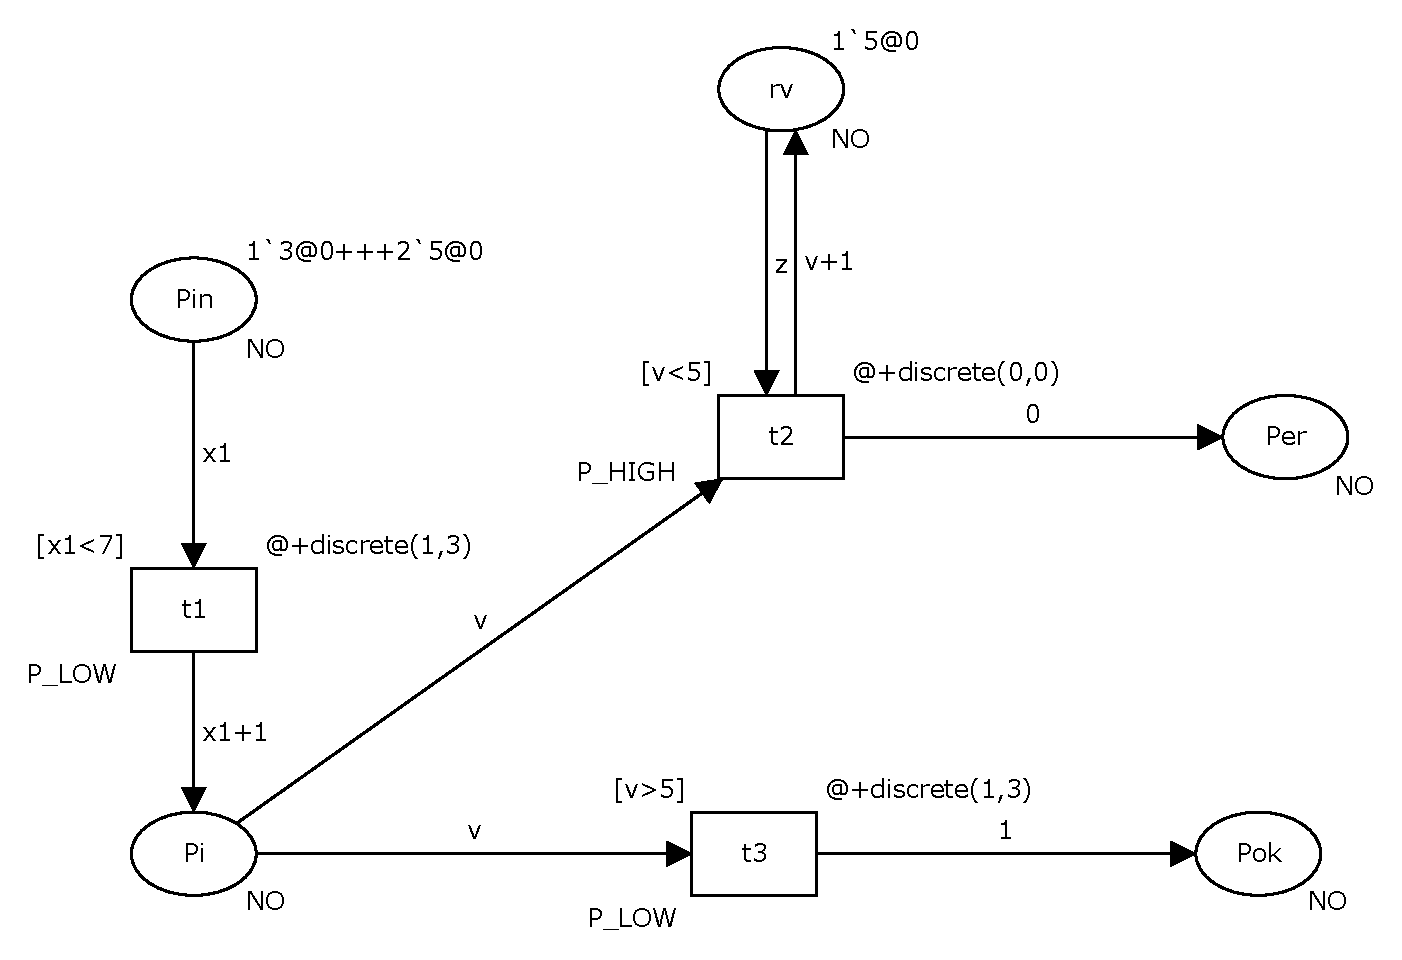
\includegraphics[width=11.5cm]{Figures/figure2_scp.eps}
% 
\caption{\label{red1}Graphical view of a PTCPN.}
\end{figure}

\begin{example} Let us consider the marked PTCPN depicted in Figure \ref{red1}, 
obtained from CPNTools examples. 
% 
Observe that timed colour tokens in CPN Tools are drawn
using the notation $n`v@x$,
meaning that we have $n$ instances of a timed colour token 
with colour value $v$ and {\em timestamp} $x$, which correspond to $n.(v,x)$
according to our formal notation. Besides, the symbol `+++'
is there used to represent the union of timed
multisets. 

Thus, $p_{\it in}$ is initially marked with one token
of colour $(3,0)$, and two tokens of colour $(5,0)$,
and the place ${\it rv}$ has one token with colour
$(5,0)$.  Transitions are labelled
with their associated guard, time interval and priority
information. 
Arcs are labelled with the corresponding expressions,
in which no time delays appear, as we are considering
that only transitions have associated time delays.

From the initial marking we can see that
only transition $t_1$ can be fired (at instant $0$), and
any token of those in $p_{\it in}$ can be used for
that purpose.  Taking $(5,0)$ we get the binding $x=5$,
which fulfils the transition guard.
The firing of $t_1$ with this binding removes
one instance of $(5,0)$ from $p_{\it in}$,
and produces a new token on $p_i$.
The timestamp of this new token is a discrete value
in the interval $[1,3]$ (let us say $3$).
Thus, considering the output
arc inscription we get a token $(6,3)$  on $p_i$.

Now, transition $t_1$ must fire again twice (until $p_{\it in}$ 
becomes empty), due to the time constraints of this model. 
As a result we may obtain in $p_i$ the following marking
$\{1.(4,3), 1.(6,1),$
$ 1.(6,3)\}$ (the timestamp values depend on the values
chosen from the interval $[1,3]$).
% 
The only transition that can be fired at this marking
is $t_3$, because due to the time constraints 
we must first use the token $(6,1)$
and $t_2$ cannot be fired using this token.
The firing of $t_3$ produces a new token on $p_{\it ok}$,
whose colour value must be $1$, and the timestamp
depends again on the chosen delay in the time interval
$[1,3]$. For instance, we could obtain the 
colour token $(1,4)$. 

Two tokens now remain in $p_i$, with colours  $(4,3)$ and 
$(6,3)$, and $t_2$ becomes the only transition
enabled (due to condition (4) of Def.\ \ref{permitidas}).
Its firing removes the token $(4,3)$ from $p_i$,
the token on the place ${\it rv}$ changes to $1.(5,3)$,  
and creates a new token on $p_{\it er}$, with colour $(0,3)$. 
%
% 
Finally, the remaining token $(6,3)$ on $p_i$ 
only allows us to fire $t_3$, generating a new token
on $p_{\it ok}$, with value $1$ and a timestamp
depending on the delay chosen for its firing.
\end{example}


%In \cite{Buc03} there is a model that
%extends Merlin's nets by including dynamic priorities and resources.
%
%The particular model that we use is also an extension of Merlin's
%nets, 
%% but it is simpler than that considered in \cite{Buc03}.
%including priorities and three transition types ({\em black,\,grey\,} and
%{\em white\,}). All transitions are assigned both a time interval
%and a static priority. The time interval restricts the instants at
%which a transition is allowed to be fired. {\em White}\, transitions
%are not forced to fire when their clock reaches its latest firing
%time, grey transitions must fire once their clock reaches that value, 
%and black  transitions
%must fire immediately, once they fulfil all the required conditions. 
%Of course, in the
%event of a conflict, any transition of those involved in the conflict 
%can be fired (whichever type it has), although we take into account 
%priorities to resolve the conflicts. Thus, priorities are only
%used in the case of conflict, when at a given marking two or more
%transitions are simultaneously enabled, then only those with 
%the maximum priority are allowed to be fired at that moment.

\section{Extended Timed-Arc Petri Nets} \label{sec:def}
%We shall now give some preliminaries in order to define the model
%of extended timed-arc Petri nets. 
%We consider only discrete time
%as for closed intervals the reachability/soundness problems
%are equivalent with the continuous time variant as discussed in 
%Section~\ref{sec:cont}.
Let $\nnul = \mathbb{N} \cup \{0\}$ and 
$\nnul^{\infty} = \nnul \cup \left\{\infty \right\}$.
A \emph{discrete timed transition system} (DTTS) 
is a triple $\left(\proc, \act,\rightarrow\right)$
where $\proc$ is the set of states, $\act$ is the set of actions
and $\rightarrow\: \subseteq \proc \times (\act \cup \nnul)  \times \proc$ is the 
transition relation written as $s \trans{a} s'$ whenever $(s,a,s') \in \rightarrow$.
If $a \in \act$ then we call it a \emph{switch transition}, if
$a \in \nnul$ we call it a \emph{delay transition}.
%By $\rightarrow^{*}$ we denote the reflexive and transitive closure of 
%the relation
%$\rightarrow  \eqdef \bigcup_{a \in \act} \trans{a} \; \cup \; \bigcup_{d \in \nnul} \trans{d}$. 
We also define the set of \emph{well-formed time intervals} as 
$\int \eqdef \{[a,b] \mid a \in \nnul,b\in \nnul^{\infty}, a\leq b \}$
and its subset $\intinv \eqdef \{[0,b] \mid b\in \nnul^{\infty} \}$
used in age invariants. 

%%% Nice intro but repeats too much from introduction, do not remove it though
%We can now introduce the timed-arc Petri net model
%where each token carries its own
%age and input arcs to transitions are annotated with time intervals
%that restrict the ages of tokens usable for transition firing. Newly
%produced tokens become of age $0$, unless they were produced by
%a pair of so-called \emph{transport arcs} that describe
%a path along which the tokens travel from input to output places 
%while preserving the ages of the tokens moved along the path. In this paper
%we study an extended model with (i) \emph{age invariants}
%associated to places that restrict the maximal possible ages of tokens
%in the given places, (ii) \emph{inhibitor arcs} that as in normal Petri
%nets inhibit transition firing, and
%(iii) \emph{urgent transitions} that disable time delay whenever
%at least one of them is enabled.
%These additional extensions add a considerable expressive power
%(as also demonstrated by the decidability and undecidability results
%proved in this paper) and they are essential for convenient modelling 
%of systems with timing attributes.

\begin{definition}[Extended timed-Arc Petri Net] \label{defetapn}  
An \emph{extended timed-arc Petri net} 
(ETAPN) is a 9-tuple $N = \tapntuple$ where 
\begin{itemize}
\item $P$ is a finite set of \emph{places},
\item $T$ is a finite set of \emph{transitions} 
such that $P \cap T = \emptyset$, 
\item $\Turg \subseteq T$ is the set of \emph{urgent transitions},
\item $\ia \subseteq P \times T$ is a finite set of \emph{input arcs},
\item $\oa \subseteq T \times P$ is a finite set of \emph{output arcs},
\item $\cfunction : \ia \rightarrow \int$ is a \emph{time constraint function} assigning 
guards %(time intervals) 
to input arcs,
\item $\wfunction : \ia\cup \oa \rightarrow \mathbb{N}$ is a function assigning \emph{weights} to input and output arcs,
\item $\type : \ia \cup \oa \rightarrow \types$ is a \emph{type function} assigning a type to all arcs where $\types = \{\normal, \inhib\} \cup \{\transporti \mid j \in \mathbb{N} \}$ such that  
\begin{itemize}
\item if $\type(a) = \inhib$ then $a \in \ia$ and $\cfunction(a)=[0,\infty]$, 
\item if $(p,t) \in \ia$ and $t \in \Turg$ then $\cfunction((p,t))=[0,\infty]$,
\item if $\type((p,t)) = \transporti$ for some $(p,t) \in \ia$ then there is exactly one $(t,p^{\prime}) \in \oa$ such that $\type((t,p^{\prime})) = 
\transporti$, 
%and moreover $\wfunction((p,t))=\wfunction((t,p^{\prime}))$,
\item if $\type((t,p^{\prime})) = \transporti$ for some $(t,p^{\prime}) \in \oa$ then there is exactly one $(p,t) \in \ia$ such that $\type((p,t)) = 
\transporti$, 
%and moreover $\wfunction((p,t))=\wfunction((t,p^{\prime}))$,
\item if $\type((p,t)) = \transporti = \type((t,p^{\prime}))$ 
then $\wfunction((p,t))=\wfunction((t,p^{\prime}))$,
\end{itemize}
\item $\inv : P \rightarrow \int^{inv}$ is a function assigning \emph{age invariants} to places.
\end{itemize}
\end{definition}

\begin{remark}
Note that for transport arcs we assume that they come in pairs (for
each type $\transporti$) so that their weights match.
Also for inhibitor arcs and for input arcs to urgent transitions, we
require that the guards are $[0,\infty]$. This restriction is important
for some of the results presented in this paper and it also guarantees that 
we can use DBM-based algorithms in the tool TAPAAL~\cite{DJJJMS:TACAS:12}.
\end{remark}

The ETAPN model is not monotonic, meaning
that adding more tokens to markings can disable time delays or
transition firing.
Therefore we define a subclass of 
ETAPN where the monotonicity breaking features are not allowed.
In the literature such nets are often considered as the standard
timed-arc Petri net model~\cite{BLT:90,Hanisch:93} but we add the 
prefix monotonic for clarity reasons. 

\begin{definition}[Monotonic timed-arc Petri net] \label{deftapn}
A \emph{monotonic timed-arc Petri net} 
(MTAPN) is an extended timed arc Petri net 
with no urgent transitions ($\Turg=\emptyset)$, no age invariants
($\inv(p) = [0,\infty]$ for all $p \in P$) and no 
inhibitor arcs ($\type(a) \not= \inhib$ for all $a \in \ia$).
\end{definition}


%Let $N = \tapntuple$ be a ETAPN and $P^\prime \subseteq P$, the projection $N|_{P^\prime}$ 
%is the net \ensuremath{(P^\prime, T, \ia^\prime,\allowbreak \oa^\prime, \cfunction^\prime, 
%\wfunction^\prime, \type^\prime, \inv^\prime)}, 
%where $\ia^\prime=\ia \cap (P^\prime \times T)$, $\oa^\prime=\oa \cap (T \times P^\prime)$,
%$\cfunction^\prime : \ia^\prime \rightarrow \int$, $\wfunction^\prime : \ia^\prime \cup \oa^\prime \rightarrow \mathbb{N}$,
%$\type^\prime : \ia^\prime \cup \oa^\prime \rightarrow \types$, and $\inv^\prime : P^\prime \rightarrow \int^{inv}$. From now on, we will denote by 
%$P_s$ the set of places shared by various nets. Then, let $N$, $N^\prime$ be two ETAPNs such that $P \cap P^\prime \subseteq P_s$, the disjoint union of $N$ and $N^\prime$ is a ETAPN \ensuremath{(P^{\prime\prime},T^{\prime\prime},\ia^{\prime\prime}, \oa^{\prime\prime},\cfunction^{\prime\prime},\wfunction^{\prime\prime},\type^{\prime\prime}, \inv^{\prime\prime})}, where $P^{\prime\prime}= P\cupdot P^\prime, T^{\prime\prime}=T\cupdot T^\prime, \ia^{\prime\prime}=\ia\cupdot \ia^\prime,\oa^{\prime\prime}=\oa \cupdot \oa^\prime,\cfunction^{\prime\prime}:\ia^{\prime\prime}\cup \oa^{\prime\prime}\rightarrow \int, \wfunction^{\prime\prime}: \ia^{\prime\prime}\cup \oa^{\prime\prime}\rightarrow \mathbb{N}, 
%\type^{\prime\prime} : \ia^{\prime\prime} \cup \oa^{\prime\prime} \rightarrow \types, \text{ and } \inv^{\prime\prime} : P^{\prime\prime} \rightarrow \int^{inv}$.

Before we give the formal semantics of the model, let us fix some notation.
Let $N = \tapntuple$ be an ETAPN. 
%Let $F\eqdef \ia \cup \oa$. 
We denote by ${}^\bullet x \eqdef 
\{y \in P \cup T \mid (y,x) \in (\ia \cup \oa),\ \type((y,x)) \neq \inhib \}$ 
the preset of a transition or a place $x$.
Similarly, the postset $x^\bullet$ is defined as 
$x^\bullet \eqdef \{y \in P \cup T \mid (x,y) \in (\ia \cup \oa) \}$.
Let $\mathcal{B}(\nnul)$ be the set 
of all finite multisets over $\nnul$. A \emph{marking} $M$ on $N$ 
is a function $M : P \longrightarrow \mathcal{B}(\nnul)$ 
where for every place $p \in P$ and 
every token $x \in M(p)$ we have $x \in \inv(p)$, in other words
all tokens have to satisfy the age invariants. 
%The projection of $P^\prime \subseteq P$ in $M$ is a function 
%$M|_{P^\prime} : P^\prime \longrightarrow \mathcal{B}(\nnul)$.
The set of all markings in a net $N$ 
is denoted by $\mathcal{M}(N)$.

We write $(p,x)$ to denote a token at a place $p$ with the 
age $x\in \nnul$. Then $M=\{(p_1,x_1),(p_2,x_2),\dots ,(p_n,x_n)\}$ 
is a multiset representing a marking $M$ with $n$ tokens of 
ages $x_i$ in places $p_i$. We 
define the size of a marking as $|M| = \sum_{p\in P}|M(p)|$ where 
$|M(p)|$ is the number of tokens located in the place $p$.

%A marked ETAPN 
%$(N,M_0)$ is a TAPN N together with an initial marking $M_0$ with all tokens of age $0$. 

\begin{definition}[Enabledness]
\label{def:enabledness}
 Let $N = \tapntuple$ be an ETAPN. 
We say that a transition $t \in T$ is \emph{enabled} in a marking $M$ by the 
multisets of tokens
$\inn = \{(p,x_{p}^1), (p,x_{p}^2), \dots ,(p,x_{p}^{\wfunction ((p,t))})\mid 
p \in {}^\bullet t\} \subseteq M$ and 
$\out = \{ (p^{\prime},x_{p^{\prime}}^1),
           (p^{\prime},x_{p^{\prime}}^2),
\dots ,\allowbreak
(p^{\prime},x_{p^{\prime}}^{\wfunction ((t,p^{\prime}))}) 
\mid p^{\prime} \in t^\bullet \}$ if
\begin{itemize}
\item for all input arcs except the inhibitor arcs, the tokens from $\inn$ satisfy the age guards of the arcs, i.e. 
%$$\forall(p,t) \in \ia, x_p^i \in \cfunction((p,t))\text{ for }1\leq i\leq w((p,t)) $$ 
$$\forall(p,t) \in \ia. \type((p,t)) \neq \inhib \Rightarrow  x_p^i \in \cfunction((p,t))\text{ for }1\leq i\leq w((p,t)) $$ 
%\item for each place $p$ in ${}^\bullet t$ there are $\wfunction ((p,t))$ tokens from $p$ in $\inn$, i.e. $$\forall p\in {}^\bullet t. \wfunction ((p,t))= n_{p} $$
%\item for each place $p^{\prime}$ in $t^\bullet $ there are $\wfunction ((t,p^{\prime}))$ tokens from $p^{\prime}$ in $\out$, i.e. $$\forall p^{\prime}\in t^\bullet . \wfunction ((t,p^{\prime}))= m_{p^{\prime}} $$
\item for any inhibitor arc pointing from a place $p$ to the
transition $t$, the number of tokens in $p$ is smaller than the weight of the arc, i.e.
$$\forall(p,t) \in \ia. \type((p,t)) = \inhib \Rightarrow|M(p)|<\wfunction ((p,t))$$ 
%$$\forall(p,t) \in \ia. \type((p,t)) = \inhib \Rightarrow \nexists x \in M(p). x \in \cfunction((p,t))$$
\item for all input arcs and output arcs which constitute a transport arc, 
the age of the input token must be equal to the age of the output token and satisfy the invariant of the output place, i.e.
\begin{eqnarray*}
&\forall(p,t) \in \ia. \forall(t,p^{\prime}) \in \oa.\type((p,t)) = \type((t,p^{\prime})) 
= \transporti \\
&\Rightarrow \big( x_p^i = x_{p^{\prime}}^i \wedge x_{p^{\prime}}^i \in 
\inv(p^{\prime})\big) \text{ for } 1\leq i \leq w((p,t))
\end{eqnarray*}
\item for all normal output arcs, the age of the output token is $0$, i.e. $$\forall(t,p^{\prime}) \in \oa. \type((t,p^{\prime})) = \normal \Rightarrow x_{p^{\prime}}^i = 0 \text{ for }1\leq i \leq w((p,t)).$$ 
\end{itemize}
\end{definition}

A given ETAPN $N$ %=\tapntuple$ 
defines a DTTS $T(N)\eqdef (\markingsof(N),T,\rightarrow)$
where states are the markings and the transitions are as follows. 
\begin{itemize}
\item If $t\in T$ is enabled in a marking $M$ by the  multisets of
tokens $\inn$ and $\out$ then $t$ can \emph{fire} and produce 
the marking $M^{\prime} = (M \smallsetminus \inn) \uplus \out$ 
where  $\uplus$ is the multiset sum operator and $\smallsetminus$ is the multiset 
difference operator; we write $M \trans{t} M^{\prime}$ for this 
switch transition.
\item A time \emph{delay} $d \in \nnul$ is allowed in $M$ if
\begin{itemize}
\item $(x+d) \in I(p)$ for all $p \in P$ and all $x \in M(p)$, and
% i.e. by delaying $d$ time units no token violates any of the age invariants, 
%and
\item if $M \trans{t} M'$ for some $t \in \Turg$ then $d=0$.
 %there is at least one urgent transition enabled in $M$ then
 %     $d=0$, i.e. enabled urgent transitions disallow time passing.
\end{itemize}
By delaying $d$ time units in $M$ we reach the marking $M^{\prime}$ defined as
$M^{\prime}(p) = \{x+d \mid x \in M(p)\}$ for all $p \in P$; 
we write $M \trans{d} M^{\prime}$ for this delay transition.
\end{itemize}

%A computation of a net $N$ from the initial marking $M_0$ is
%$M_0 \rightarrow M_1\rightarrow \cdots \rightarrow M_n$ is 
%denoted by $\{M_i\}_{i=0}^{n}$ 
%and we call it a \emph{run}. If the sequence is infinite, we write 
%$\{M_i\}_{i\geq 0}$. Moreover, we write $M \Rightarrow^* M^{\prime}$ if  
%$M^{\prime}$ is reachable from $M$ and $[M\rangle$ represents the set of reachable markings of $M$.

\noindent Let 
$\trans{} \eqdef \bigcup_{t \in T} \trans{t} \cup \bigcup_{d \in \nnul} \trans{d}$.
The set of all markings reachable %in the net $N$ 
from a given marking $M$ is denoted by 
$[M\rangle \eqdef \{ M' \mid M \trans{}^* M' \}$.
By $M \trans{d,t} M'$ we denote that there is a marking $M''$
such that $M \trans{d} M'' \trans{t} M'$.

A marking $M$ is a \emph{deadlock} if there is no $d \in \nnul$ and
no $t \in T$ such that $M \trans{d,t} M'$ 
for some marking $M'$.
A marking $M$ is \emph{divergent} if for any $d \in \nnul$
we have $M \trans{d} M'$ for some $M'$.


%\section{Finite Abstractions for Bounded ETAPNs}

In general, ETAPNs are infinite in two dimensions. The number of tokens
in reachable markings can be unbounded and even for bounded nets
the ages of tokens can be arbitrarily large. We shall now recall a 
few results that allow us to make finite abstractions for bounded
ETAPNs, i.e. for nets where the maximum number of tokens in any
reachable marking is bounded by a constant.

Let $N=\tapntuple$ be a given ETAPN.
In~\cite{ALSST:MEMICS:12} 
the authors provide an algorithm for computing 
a function $\cmax: P \rightarrow (\nnul \cup \{ -1 \})$ 
returning for each place $p \in P$ the maximum constant associated
to this place, meaning that the ages of tokens in place $p$ that
are strictly greater than $\cmax(p)$ are irrelevant. In particular,
places where $\cmax(p)=-1$ are the so-called \emph{untimed} places
where the age of tokens is not relevant at all, implying that all
the intervals on their ongoing arcs are $[0,\infty]$.

Let $M$ be a marking of $N$. We split it into 
two markings $\mold$ and $\myoung$ where 
$\mold (p)=\left\{ x\in M(p) \mid x>\cmax(p) \right\}$ 
and $\myoung (p)=\allowbreak\left\{ x\in M(p) \mid 
x\allowbreak\leq\allowbreak \cmax(p) \right\}$
for all places $p \in P$. Clearly,
$M = \mold \uplus \myoung$.

We say that two markings $M$ and $M'$ in the net $N$ are equivalent, 
written $M \eqMarking M^{\prime}$, 
if $\myoung=\myoung^{\prime}$
and for all $p \in P$ we have
$|\mold (p)|=|\mold^{\prime}(p)|$.
In other words $M$ and $M'$ agree on the tokens with ages below the
maximum constants and have the same number of tokens above the maximum
constant.
% (relevant only for places $p$ with $I(p)=[0,\infty]$ as
%places with nontrivial age invariants cannot have tokens older that 
%the maximum constant which is in this case equal to the invariant upper-bound).

The relation $\eqMarking$ is an equivalence relation and it is
also a timed bisimulation 
where delays and transition firings on one side can be matched by
exactly the same delays and transition firings on the other side
and vice versa. % (see e.g.~\cite{LY:97}).

\begin{theorem}[\cite{ALSST:MEMICS:12}]
\label{thm:bisim}
  The relation $\eqMarking$ is a timed bisimulation.
\end{theorem}

We can now define canonical representatives for each
equivalence class of $\eqMarking$. 

\begin{definition}[Cut]
\label{def:cut}
Let $M$ be a marking.
We define its canonical marking $\cut(M)$ by 
$\cut(M)(p)= \myoung(p)\uplus \big\{ \underbrace{ \cmax(p)+1,\dots ,\cmax(p)+1 }_{|\mold(p)| \text{ times}} \big\}$.
%\begin{equation*}
%  \cut(M)(p)=
%\begin{cases}
%\myoung(p)  \quad \text{if $p$ is invariant or dead-token place,} \\
%\myoung(p)\uplus \big\{ \underbrace{ \cmax(p)+1,\dots ,\cmax(p)+1 }_{|\mold(p)| \text{ times}} \big\}    \quad \text{if $p$ is a normal place.}
%\vspace{-.45cm}
%\end{cases}
%\vspace{.45cm}
%\end{equation*}
\end{definition}

\begin{lemma}[\cite{ALSST:MEMICS:12}]
\label{lemma:canon}
Let $M$, $M_1$ and $M_2$ be markings. Then
(i) $M \eqMarking \cut(M)$, and (ii)
$M_1 \eqMarking M_2$ if and only if $\cut(M_1)=\cut(M_2)$.
\end{lemma}

Let $M$ and $M^\prime$ be two markings. We say that $M^\prime$ \emph{covers} 
$M$, denoted by $M \sqsubseteq M^\prime$, if $M(p) \subseteq M^\prime(p)$ 
for all $p \in P$. We write $M \sqsubseteq_{cut} M^\prime$ 
if $cut(M) \sqsubseteq cut(M^\prime)$.

For monotonic timed-arc Petri nets we can now show that adding more tokens
to the net does not restrict its possible behaviour. 

\begin{lemma}
\label{lem:mono}
Let $N$ be an MTAPN and $M,M' \in \mathcal{M}(N)$
be two of its markings such that $M \sqsubseteq_{\cut} M'$. 
If $M \trans{d} M_1$ (resp. $M \trans{t} M_1$) then 
$M' \trans{d} M'_1$ (resp. $M' \trans{t} M'_1$) such that 
$M_1 \sqsubseteq_{cut} M'_1$ and 
$|M'|-|M|=|M'_1|-|M_1|$.
\end{lemma}
\begin{proof}
Let $M \trans{d} M_1$, resp. $M \trans{t} M_1$.
As $M \equiv \cut(M)$ by Lemma~\ref{lemma:canon}(i),
we can by Theorem~\ref{thm:bisim} conclude that also $\cut(M) \trans{d} M_2$,
resp. $\cut(M) \trans{t} M_2$,
such that $M_1 \equiv M_2$. Recall that $\cut(M) \sqsubseteq \cut(M')$
by the assumption of the lemma.
\begin{itemize}
\item Time delay case ($\cut(M) \trans{d} M_2$).
As the net does not contain any nontrivial age invariants
and there are no urgent transitions,
we know that also $\cut(M') \trans{d} M_3$ such that
$M_2 \sqsubseteq M_3$ as time delay preserves the $\sqsubseteq$-relation.
\item Transition firing case ($\cut(M) \trans{t} M_2$).
As the net does not have any inhibitor arcs,
we can see that also $\cut(M') \trans{t} M_3$ by consuming
exactly the same tokens in $\cut(M')$ as we did in $\cut(M)$.
Clearly, $M_2 \sqsubseteq M_3$.
\end{itemize}
Because $\cut(M') \equiv M'$ due to Lemma~\ref{lemma:canon}(i),
we know by Theorem~\ref{thm:bisim}
that $M' \trans{d} M'_1$, resp. $M' \trans{t} M'_1$, such that $M_3 \equiv M'_1$.
Hence $M_1 \equiv M_2 \sqsubseteq M_3 \equiv M'_1$.
By Lemma~\ref{lemma:canon}(ii) we get
$\cut(M_1)=\cut(M_2)$ and $\cut(M_3)=\cut(M'_1)$.
Observe now a simple fact that $M_2 \sqsubseteq M_3$ implies that
$\cut(M_2) \sqsubseteq \cut(M_3)$.
This all together implies that $\cut(M_1)=\cut(M_2) \sqsubseteq
\cut(M_3) = \cut(M'_1)$ which is another way of saying that
$M_1 \sqsubseteq_\cut M'_1$ as required by the lemma.
As time delays do not change the number of
tokens in $M$ and $M'$ and transition firing adds or removes an
equal number of tokens from both $M$ and $M'$,
we can also conclude that $|M'|-|M|=|M'_1|-|M_1|$.
\qed
\end{proof}




